\documentclass[a4paper]{article}
\usepackage{tikz}
\usetikzlibrary{petri,arrows}
\usepackage{amstext}

\begin{document}


%% TikZ style options %%
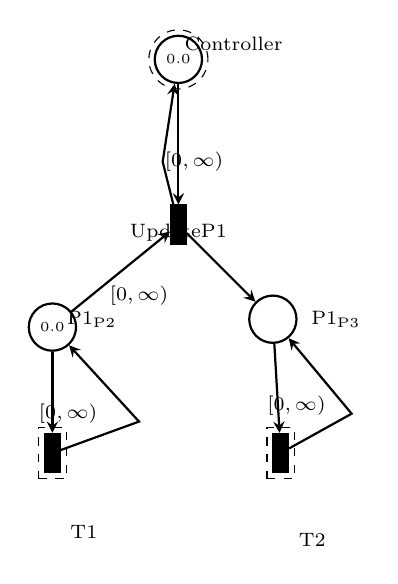
\begin{tikzpicture}[font=\scriptsize, xscale=1, yscale=1]
%% the figure can be scaled by changing xscale and yscale
%% positions of place/transition labels that are currently fixed to label=135 degrees
%% can be adjusted so that they do not cover arcs
%% similarly the curving of arcs can be done by adjusting bend left/right=XX
%% labels may be slightly skewed compared to the tapaal drawing due to rounding.
%% This can be adjusted by tuning the coordinates of the label
\tikzstyle{arc}=[->,>=stealth,thick]
\tikzstyle{transportArc}=[->,>=diamond,thick]
\tikzstyle{inhibArc}=[->,>=o,thick]
\tikzstyle{every place}=[minimum size=6mm,thick]
\tikzstyle{every transition} = [fill=black,minimum width=2mm,minimum height=5mm]
\tikzstyle{every token}=[fill=white,text=black]
\tikzstyle{sharedplace}=[place,minimum size=7.5mm,dashed,thin]
\tikzstyle{sharedtransition}=[transition, fill opacity=0, minimum width=3.5mm, minimum height=6.5mm,dashed]
\tikzstyle{urgenttransition}=[place,fill=white,minimum size=2.0mm,thin]\tikzstyle{uncontrollabletransition}=[transition,fill=white,draw=black,very thick]
%% TikZ-figure elements %%
\node[place, structured tokens={0.0},] at (3.9,-1.4) (Controller) {};
\node[sharedplace] at (Controller.center) { };
%% label for place Controller
\draw (4.6,-1.2) node[align=left] {$\mathrm{Controller}$};
\node[place, structured tokens={0.0},] at (2.3,-4.8) (P1_P2) {};
%% label for place P1_P2
\draw (2.8,-4.7) node[align=left] {$\mathrm{P1_{P2}}$};
\node[place] at (5.1,-4.7) (P1_P3) {};
%% label for place P1_P3
\draw (5.9,-4.7) node[align=left] {$\mathrm{P1_{P3}}$};
\node[transition] at (3.9,-3.5) (UpdateP1) {};
%% label for transition UpdateP1
\draw (3.9,-3.6) node  {$\mathrm{UpdateP1}$};
\node[transition] at (2.3,-6.4) (T1) {};
\node[sharedtransition] at (T1.center) { };
%% label for transition T1
\draw (2.7,-7.4) node  {$\mathrm{T1}$};
\node[transition] at (5.2,-6.4) (T2) {};
\node[sharedtransition] at (T2.center) { };
%% label for transition T2
\draw (5.6,-7.5) node  {$\mathrm{T2}$};
\draw[arc] (P1_P2) to[bend right=0] (T1) {};
%% Label for arc between P1_P2 and T1
\draw (2.5,-5.9) node {$\mathrm{[0,\infty)}$};
\draw[arc] (T1) to[bend right=0] (3.4,-6.0) to[bend right=0] (P1_P2) {};
\draw[arc] (P1_P3) to[bend right=0] (T2) {};
%% Label for arc between P1_P3 and T2
\draw (5.4,-5.8) node {$\mathrm{[0,\infty)}$};
\draw[arc] (T2) to[bend right=0] (6.1,-5.9) to[bend right=0] (P1_P3) {};
\draw[arc] (UpdateP1) to[bend right=0] (P1_P3) {};
\draw[arc] (P1_P2) to[bend right=0] (UpdateP1) {};
%% Label for arc between P1_P2 and UpdateP1
\draw (3.4,-4.4) node {$\mathrm{[0,\infty)}$};
\draw[arc] (Controller) to[bend right=0] (UpdateP1) {};
%% Label for arc between Controller and UpdateP1
\draw (4.1,-2.7) node {$\mathrm{[0,\infty)}$};
\draw[arc] (UpdateP1) to[bend right=0] (3.7,-2.7) to[bend right=0] (Controller) {};
\end{tikzpicture}
\end{document}
